%-------------------------------------------------------------------------------
\section{Preliminary Results}
%-------------------------------------------------------------------------------



In order to explore evidence for the case for \sys{}, we ask the following
questions: 
\begin{enumerate}
    \item How does function latency in \sys{} compare to schedulers without
    priorities?
    \item Does \sys{}'s plan for managing memory work?
\end{enumerate}


To explore these questions, we build a simulator in go\cite{golang}, which
simulates different scheduling approaches. Using a simulator allows us to extend
the experiments to include many more machines than would otherwise be available
to us.

\begin{figure}[t!]
    \centering
      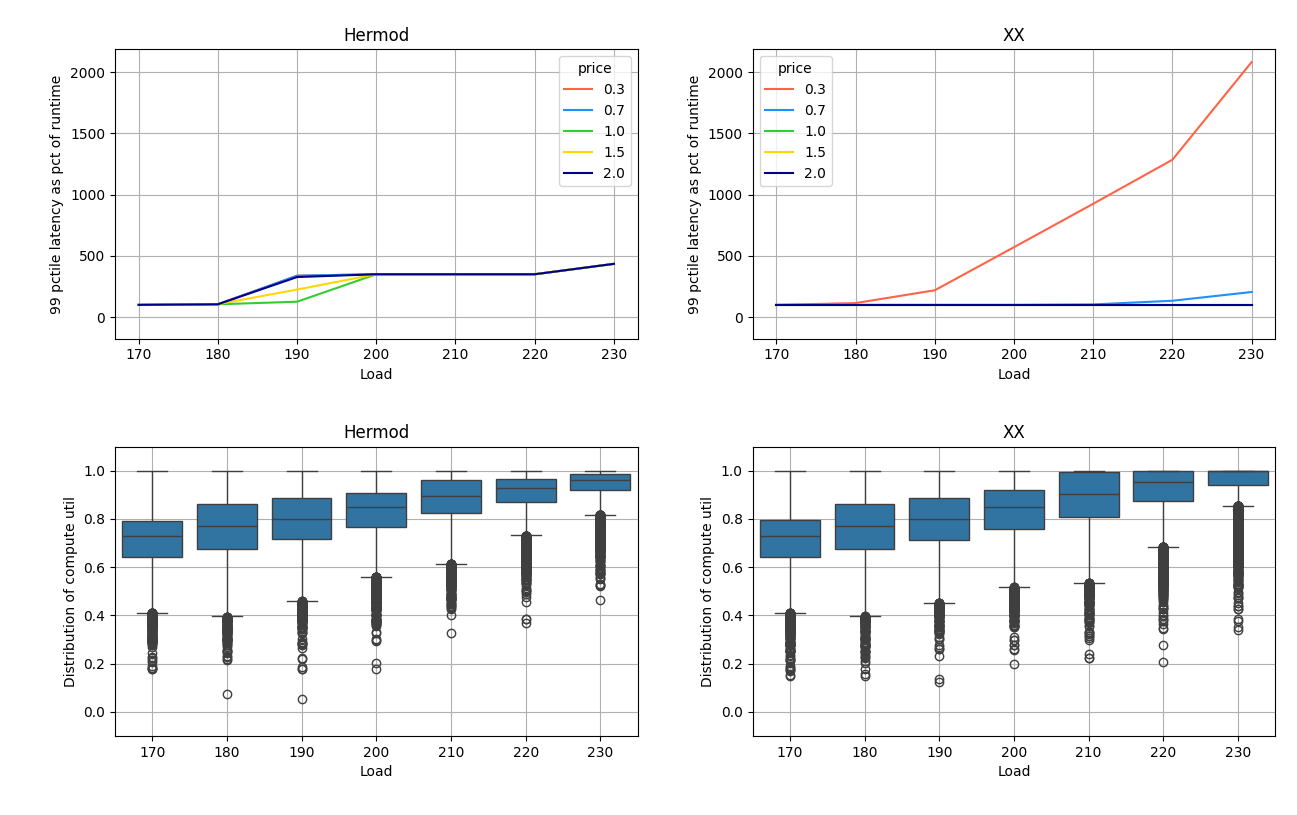
\includegraphics[width=8.5cm]{img/hermod_xx_latencies.png}
      \caption{ tail latency distribution and compute utilization for Hermod and
      \sys{}. At tick 50 (left right line) the load was increased, and at tick
      80 (right red line) it was decreased again }
    \label{fig:hermod-xx-edf}
\end{figure}


\subsection{Experimental Setup}

In each version of the simulator, functions arrive in an open loop at a given
rate. The simulator attaches three main characteristics to each function it
generates: runtime, \priceclass{}, and memory usage.\ \textit{Function runtime}
is chosen by sampling from randomly generated long tailed (in this case pareto)
distribution: the relative length of the tail ($\alpha$ value) remains constant,
and the minimum value ($x_m$) is chosen from a normal distribution. This process
for sampling reflects the fact that different functions have different expected
runtimes (chosen from a normal distribution), and that actual invocation
runtimes follow long tailed distributions (so each pareto distribution that we
sample represents the expected runtime distribution of a given function).\
\textit{Function \class{}} is chosen randomly, but weighted: the simulator uses
a bimodal weighting across priorties. The simulator has $n$ different
\priceclass{} values, each assigned to a fictitious price. Because functions are
randomly assigned a \class{}, runtime and \class{} are not correlated.\
\textit{Function memory usage} is chosen randomly between 100MB and 10GB. Over
their lifetime, functions increase their memory usage from an initial amount
(always 100MB) to their total usage.

When comparing two different simulated schedulers, they each are given an
identical workload and then each simulate running that workload.

The simulator makes some simplifying assumptions:
\begin{enumerate}
    \item functions are compute bound, and do not block for i/o
    \item communication latencies are not simulated
    \item the amount of time it takes to swap memory is not simulated
\end{enumerate}

We simulate running 100 machines with 8 cores each, 4 scheduler shards, and a
k-choices value of 3 when applicable.

\subsection{How do function latencies compare?}

The goal of \sys{} is to reduce the variance of latencies for high \priceclass{}
functions. This experiment shows that \sys{} is able to do this even under
varying load, and compares \sys{}'s performance to a scheduler that does not
take into account any information about which functions are latency sensitive.

We compare \sys{} performance to that of an existing scheduler that does not
take priority into account. We simulate Hermod\cite{hermod}, a state-of-the-art
research scheduler built specifically for serverless. Hermod's design is the
result of a from-first-principles analysis of different scheduling paradigms. In
accordance with the paper's findings, we simulate least-loaded load balancing
over machines found using power-of-k-choices, combined with early binding and
Processor Sharing machine-level scheduling. Hermod does not use priorities in
its design, and as such the simulator ignores functions' \class{} when
simulating Hermod's design.

Because Hermod does not deal with memory pressure, and to avoid an unfair
comaprison with \sys{}'s swapping, we set the memory to be absurdly high for all
\sys{} as well as Hermod in this experiment. We also turn off the use of the
idle list in \sys{}, so as to be on par with Hermod in placing load, and revert
solely to k-choices.

We begin with a medium load setting, and then increase the load to more than a
steady setting cand handle for a window of time. A strong result for \sys{}
would show that it is able to maintain low latency for high \priceclass{}
functions, even under the high load. Figure~\ref{fig:hermod-xx-edf} shows the
results. We can see that \sys{} is indeed able to maintain low latencies for the
high \class{} functions. Hermod spreads the performance degradation across all
the different functions, and as a result all of their latencies go up equally.


\subsection{Does \sys{} plan for memory management work?}

\begin{figure}[t!]
    \centering
      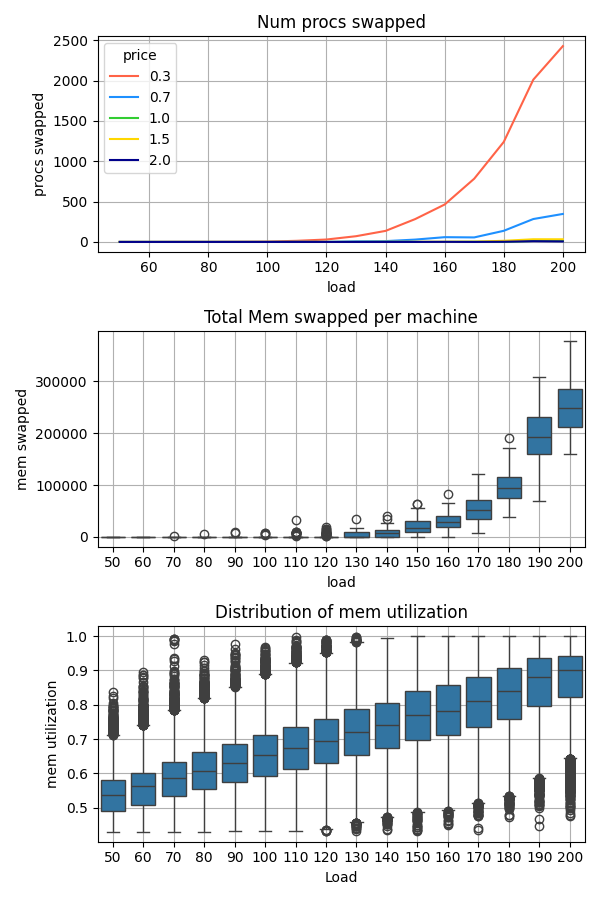
\includegraphics[width=8cm]{img/memory_graphs.png}
      \caption{ \sys{}'s swapping behavior. The amount of memory is in MB  }
    \label{fig:memory-graphs}
\end{figure}

To answer this question, we look at how \sys{} distributes load, and whether the
amount that \sys{} needs to swap memory is realistic. We now run \sys{} in a
setting of limited memory (32GB of RAM per machine), and track the memory
utilization of different machines, as well as how much and what machines need to
swap. A good result would show: a small spread of memory utilization, that
machines only start swapping once memory utilization is high, and that the
amount of swapping being done is equally spread across machines.
Figure~\ref{fig:memory-graphs} shows the results. We can see \sys{} swaps only
lower \class{} functions' memory, and that the amount of memory swapped is faily
evenly distributed between all the machines. We can also conclude that with a
500GB SSD, a provider would comfortably be able to avoid killing while running
the datacenter at an average memory utilization of $\sim$90$\%$, at the cost of
$\sim\$$30 per machine for swap space~\cite{ssd-price}.


